\appendix
\begin{center}
{
\Large
\textbf{
Deep Learning for Two-Sided Matching}
~\\
~\\	
Appendix
}
\end{center}


\section{RSD is not Stable}\label{app:rsd-unstable}
In the following example, we show RSD mechanism is not stable.

\begin{example}
\label{ex:1}
Consider $n = 3$ workers and $m = 3$ firms with the following preference orders:
\begin{align*}
    w_1: f_2, f_3, f_1, \bot \quad f_1: w_1, w_2, w_3, \bot\\
    w_2: f_2, f_1, f_3, \bot \quad f_2: w_2, w_3, w_1, \bot\\
    w_3: f_1, f_3, f_2, \bot \quad f_3: w_3, w_1, w_2, \bot
\end{align*}
The  matching found by worker-proposing DA is $(w_1, f_3), (w_2, f_2), (w_3, f_1)$. This is a stable matching. If $f_1$ truncates and misreports its preference as $f_1: w_1, w_2, \bot, w_3$, the matching found is $(w_1, f_1), (w_2, f_2), (w_3, f_3)$. Firm $f_1$ is matched with a more preferred worker, and hence the mechanism is not strategy-proof.
%
Now consider the matching under RSD. The marginal matching probabilities $r$ is given by: 
\begin{equation*}
r = 
\left(\begin{matrix}
\frac{11}{24} & \frac{1}{4} & \frac{7}{24}\\[4pt]
\frac{1}{6} & \frac{3}{4} & \frac{1}{12}\\[4pt]
\frac{3}{8} & 0 & \frac{5}{8} 
\end{matrix}\right)
\end{equation*}

$f_2$ and $w_2$ are the most preferred options for $w_2$ and $f_2$ respectively and they would prefer to be matched with each other always rather than being fractionally matched with each other. Here $(w_2, f_2)$ is a blocking pair and thus RSD is not stable.
\end{example}


\section{Proof of Theorem~\ref{thm:regret}}\label{app:omitted-proofs}
\begin{proof}
Since $\mathit{regret}(g^\theta, \succ)\geq 0$ then $\mathit{RGT}(g^\theta)=\mathbb{E}_{\succ} \mathit{regret}(g^\theta,\succ)=0$ if and only if 
$\mathit{regret}(g^\theta, \succ)= 0$  \sloppy except on zero measure events. 
Moreover, $\mathit{regret}(g^\theta, \succ)= 0$ implies $\mathit{regret}_w(g^\theta, \succ) = 0$ for any worker $w$ and $\mathit{regret}_f(g^\theta, \succ) = 0$ for any firm $f$. For each worker $w$, by definition of $\mathit{regret}_w(g^\theta, \succ)$ (Eq.~(\ref{eq:regret-worker})), $\sum_{f\in F: f\succ_w f'} g_{wf}(\succ_w, \succ_{-w}) \geq \sum_{f\in F: f\succ_w f'} g_{wf}(\succ'_w, \succ_{-w})$ and similar result holds for each firm $f$. Then $g^\theta$ is FOSD-SP. If $g^\theta$ is FOSD-SP, it is straightforward to show that $\mathit{regret}(g^\theta, \succ)= 0$.
\end{proof}


\section{Training Details}\label{app:train-detail}

For all our settings, we use a neural network with $R = 4$ hidden layers with 256 hidden nodes each. We use the leaky ReLU activation function at each of these layers. To train our neural network, we use the Adam Optimizer with decoupled weight delay regularization (implemented as AdamW optimizer in PyTorch) We set the learning rate to $0.005$ for uncorrelated preferences setting and $0.002$ when $p_{corr} = \{0.25, 0.5, 0.75\}$. The remaining hyperparamters of the optimizer are set to their default values. We sample a fresh minibatch of 1024 profiles and train our neural networks for a total of 50000 minibatch iterations. We reduce the learning rate by half once at $10000^{th}$ iteration and once at $25000^{th}$ iteration. We report our results on 204800 preference profiles.

For our training, we use a single Tesla V-100 GPU. For each setting, the neural network takes 4.6 hours to train.

\section{Additional Experiments}\label{app:additional-experiments}

In addition to the experiments in Section \ref{sec:experiments}, we also consider the following matching environments:
\begin{itemize}[leftmargin=*]
\item $n = 4$ workers and $m = 4$ firms with correlated preference with $p_{\mathrm{corr}} = 0.25$ and no truncation.
\item $n = 4$ workers and $m = 4$ firms with correlated preference with $p_{\mathrm{corr}} = 0.25$ and but preferences are truncated with $p_{\mathrm{trunc}} = 0.5$
\end{itemize}
\begin{figure}[h!]
\centering
\begin{subfigure}[b]{0.49\textwidth}
\centering
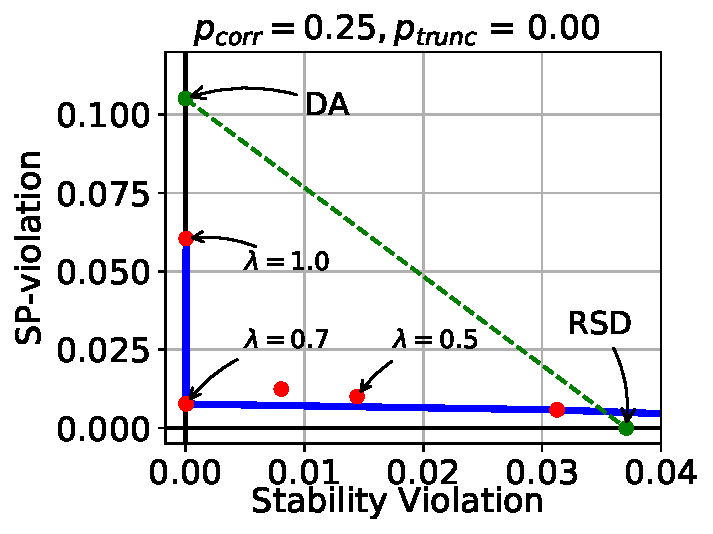
\includegraphics[scale=0.5]{plots/p_0.00_corr_0.25.pdf}
\end{subfigure}
\begin{subfigure}[b]{0.49\textwidth}
\centering
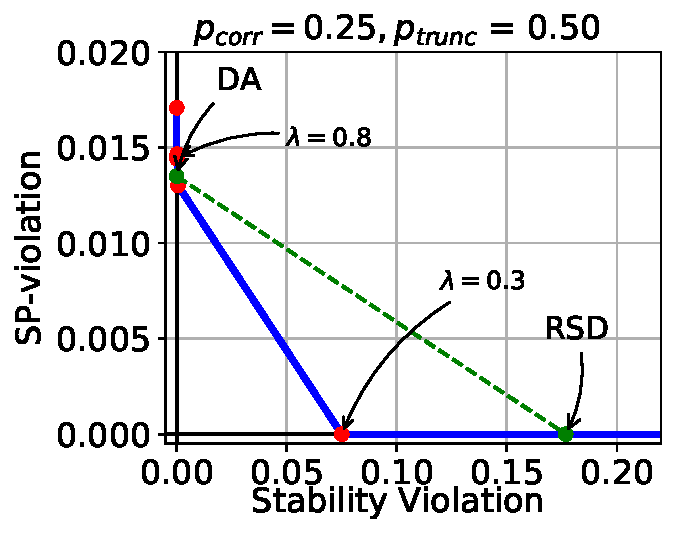
\includegraphics[scale=0.5]{plots/p_0.50_corr_0.25.pdf}
\end{subfigure}
\caption{\label{fig:frontier_add} Comparing stability violation and strategy-proofness violation from the learned mechanisms for different choices of $\lambda$ (red dots) with the best of worker- and firm-proposing DA, as well as RSD, in 4x4 two-sided matching, with correlated preference ($p_{\mathrm{corr}} = 0.25$) for different values of truncation probability. The stability violation for RSD includes IR violations.}
\vspace{-10pt}
\end{figure}

We plot the resulting frontier for both these settings in Figure~\ref{fig:frontier_add}.